\chapter{บทนำ}
\section{ที่มาและความสำคัญ}
	ปัจจุบันนี้ปัญหาภาวะโลกร้อนนั้นเป็นปัญหาใหญ่ที่ทั้งโลกกำลังให้ความสำคัญและ\\พยายามที่จะช่วยกันแก้ไขปัญหานี้เพราะด้วยปัญหาภาวะโลกร้อนนี้ส่งผลกระทบมากในหลายๆด้านไม่ว่าจะเป็นระบบนิเวศที่เปลี่ยนแปลง ภูมิอากาศระดับน้ำทะเลที่กำลังเพิ่มสูงขึ้น  ซี่งปรากฏการณ์ทั้งหลายเกิดจากภาวะโลกร้อนขึ้นที่มีมูลเหตุมาจากการปล่อยก๊าซพิษต่างๆ จากโรงงานอุตสาหกรรม จากควันท่อไอเสียของยานยนต์ การเผาขยะ ทำให้แสงอาทิตย์ส่องทะลุผ่านชั้นบรรยากาศมาสู่พื้นโลกได้มากขึ้น ซึ่งนั่นเป็นที่รู้จักกันโดยเรียกว่า สภาวะเรือนกระจก \cite{mitchell1989greenhouse} ทั้งนี้เราจึงพยายามแก้ปัญหาด้วยการใช้พลังงานทดแทนเพื่อลดมลภาวะเช่น พลังงานไฟฟ้า พลังงานแสงอาทิตย์ พลังงานลม พลังงานจากชีวภาพ และวิธีการนำพลังงานทดแทนเหล่านี้ไปใช้ได้ถูกประยุกต์ให้ใช้ได้ทุกๆส่วนของชีวิตเรามากขึ้นเช่น การใช้พลังงานแสงอาทิตย์มาผลิตไฟฟ้าเพื่อใช้ในบ้านและยานยนต์ไฟฟ้าเป็นต้น ซึ่งยานยนต์ไฟฟ้าในขณะนี้กำลังได้รับความนิยมเป็นอย่างมาก \cite{cazzola2016global},
	\cite{ding2022integrating} แต่ก็มีปัญหาในด้านประสิทธิภาพที่ต้องได้รับการพัฒนาต่อไปและส่วนประกอบที่สำคัญมากสำหรับยานยนต์ ไฟฟ้าที่ต้องพัฒนาเป็นอันดับต้นๆนั่นก็คือส่วนที่ใช้ในการกักเก็บพลังงานไฟฟ้าเพื่อให้ยานยนต์ ไฟฟ้านั้นเอาพลังงานไฟฟ้าไปใช้ในการขับเคลื่อนส่วนประกอบต่างๆต่อไปก็คือแบตเตอรี่ ซึ่งแบตเตอรี่นั้นมีปัจจัยหลายอย่างมากที่จะต้องนำมาพิจารณาเช่น อุณหภูมิ ขนาด น้ำหนัก พลังงานที่กักเก็บได้ การชาร์จ การดิสชาร์จ เป็นต้นและปัจจัยเหล่านี้ส่งผลกระทบกับยานยนต์ไฟฟ้าโดยตรงซึ่งแบตเตอร์รี่ที่ได้รับความนิยมมากในขณะนี้คือลิเธียมไอออน\\(Lithium-Ion Battery) เนื่องจากให้พลังงานที่สูงและยังสามารถเก็บพลังงานได้มากด้วยเช่นกัน มีอายุการใช้งานที่นาน ขนาดเล็ก น้ำหนักเบา มีความเสถียรซึ่งเหมาะกับการนำไปใช้สำหรับยานยนต์ไฟฟ้าอย่างมากเมื่อเทียบกับแบตเตอรี่ชนิดอื่นๆเช่น แบตเตอรี่ลิเธียมโพลิเมอร์(Li-Po) และแบตเตอรี่ตะกั่วกรด(Lead-Acid)\cite{miao2019current},\cite{wang2019reliability} และแบตเตอรี่ลิเธียมไอออนนั้นมีหลายประเภทตามส่วนประกอบทางเคมีภายในตัวแบตเตอรี่ยกตัวอย่างเช่น Lithium Cobalt Oxide
	$(LiCoO2)$, Lithium Nickel Oxide\\$(LiNiO2)$, Lithium Iron Phosphate$(LiFePO4)$ และ Lithium Nickel Manganese Cobalt Oxide\\$(Li(Ni_xMn_yCo_{1−x−y})O2$ ซึ่งในส่วนประกอบเหล่านี้จะทำให้ได้ข้อดีและข้อเสียที่ต่างกัน\cite{miao2019current}
\newline 
\hspace*{2cm} แบตเตอรี่ที่นำไปใช้สำหรับยานยนต์ นั้นจำเป็นจะต้องได้รับมาตรฐานที่เชื่อถือได้เพื่อความปลอดภัยของทั้งผู้ขับขี่และผู้โดยสารดังนั้นผู้ผลิตจึงจำเป็นจะต้องทำการทดสอบแบตเตอรี่ก่อนที่จะนำมาใช้กับยานยนต์ ไฟฟ้าตามมาตรฐานสากลที่ได้รับการยอมรับยกตัวอย่างเช่น IEC, ISO,UN ECE R100 เป็นต้นโดยแต่ละมาตรฐานนั้นก็จะมีวิธีการทดสอบและเกณฑ์ที่แตกต่างกันออกไปเช่นการทดสอบความทนต่ออุณหภูมิมาตรฐาน UN 38.3:2015 นั้นจะทดสอบแบตเตอรี่จะเก็บแบตเตอรี่ที่อุณหภูมิ $75\pm 2^{\circ}C$  อย่างน้อย 6 ชั่วโมง(12 ชั่วโมงสำหรับแบตเตอรี่ขนาดใหญ่) และจากนั้นก็นำไปเก็บที่อุณหภูมิ $-40\pm 2^{\circ}C$ โดยให้เวลาพักแบตเตอรี่มากสุด 30 นาทีและทำซ้ำจนครบ 10 cycle ส่วน IEC 62133-2:2017 นั้นนำแบตเตอรี่อยู่ในอุณหภูมิ $70\pm 2^{\circ}C$ เป็นเวลา 7 ชั่วโมงโดยที่ตัวถังของแบตเตอรี่ต้องไม่รบกวนผลของการป้องกันภายในของส่วนประกอบต่างๆของแบตเตอรี่\cite{ruiz2018review} ซึ่งจะเห็นได้ชัดถึงความแตกต่างของวิธีการทดสอบและความยากง่ายของการทดสอบ ในประเทศไทยเองก็จะมีมาตรฐานในการทดสอบแบตเตอรี่เช่นกันคือ มอก. ซึ่งมอก.เป็นคํายอมาจาก "มาตรฐานผลิตภัณฑ์อุตสาหกรรม" หมายถึงกําหนดทางวิชาการที่สำนักงานมาตรฐานผลิตภัณฑ์อุตสาหกรรม(สมอ.)ได้
\\กําหนดขึ้นเพื่อเป็นแนวทางแก่ผู้ผลิตในการผลิตสินค้าให้มีคุณภาพในระดับที่เหมาะสมกับการใช้งานมากที่สุดโดยจัดทำออกมาเป็นเอกสารและจัดพิมพ์เป็นหนังสือภายในมอก.แต่ละเล่มประกอบด้วยเนื้อหาที่เกี่ยวข้องกับการผลิตผลิตภัณฑ์นั้นๆ 
เช่น เกณฑ์ทางเทคนิค คุณสมบัติที่สําคัญ ประสิทธิภาพของการนําไปใช้งาน คุณภาพของวัสดุที่นํามาผลิตและวิธีการทดสอบเป็นต้น
\newline 
\hspace*{2cm} โครงงานวิศวกรรมไฟฟ้านี้ได้นำเสนอการทดสอบแบตเตอรี่โดยอ้างอิงมาตรฐานสากลและมาตรฐานในประเทศไทยเพื่อสำหรับนำไปประยุกต์ใช้และพัฒนายานยนต์ไฟฟ้าต่อไป โดยโครงงานนี้จะเลือกใช้แบตเตอรี่ชนิด Lithium nickel manganese cobalt oxide (NMC) และเครื่องทดสอบแบตเตอรี่ Chroma Model 17020 ในการทดสอบ
%------------------------------------------------------------------------------------------
\section{วัตถุประสงค์ของโครงงาน}
\begin{itemize}
  \item เพื่อศึกษาแนวทางในการทดสอบแบตเตอรี่
  \item เพื่อทดสอบแบตเตอรี่ชนิด Lithium nickel manganese cobalt oxide (NMC)
  \item เพื่อนำแนวทางในการทดสอบแบตเตอรี่นี้ไปประยุกต์ใช้ในยานยนต์ไฟฟ้า
\end{itemize}
%------------------------------------------------------------------------------------------
\section{ขอบเขตการทำงาน}
ทดสอบการชาร์จดิสชาร์จของแบตเตอรี่ NMC โดยใช้เครื่องทดสอบแบตเตอรี่ Chroma Model 17020 ในการทดสอบแบตเตอรี่
%------------------------------------------------------------------------------------------
\section{ขั้นตอนการดำเนินงาน}
\begin{center}
%\begin{table}[]
%\caption{ตารางแสดงขั้นตอนการดำเนินงาน}
%\centering
%\resizebox{\textwidth}{!}{%
%\begin{tabular}{|l|l|l|l|l|l|l|l|l|l|l|}
%\hline
%\multicolumn{1}{|c|}{\textbf{\Huge การดำเนินงาน}} &
%  \multicolumn{1}{c|}{\textbf{\Huge ส.ค.-65}} &
%  \multicolumn{1}{c|}{\textbf{\Huge ก.ย.-65}} &
%  \multicolumn{1}{c|}{\textbf{\Huge ต.ค.-65}} &
%  \multicolumn{1}{c|}{\textbf{\Huge พ.ย.-65}} &
%  \multicolumn{1}{c|}{\textbf{\Huge ธ.ค.-65}} &
%  \multicolumn{1}{c|}{\textbf{\Huge ม.ค.-66}} &
%  \multicolumn{1}{c|}{\textbf{\Huge ก.พ.-66}} &
%  \multicolumn{1}{c|}{\textbf{\Huge มี.ค.-66}} &
%  \multicolumn{1}{c|}{\textbf{\Huge เม.ย-66}} &
%  \multicolumn{1}{c|}{\textbf{\Huge พ.ค.-66}} \\[5ex] \hline
%{\huge ศึกษาข้อมูลเกี่ยวกับแบตเตอรี่ NMC และมาตรฐานต่างๆในการทดสอบแบตเตอรี่ \par} &
%  \cellcolor[HTML]{92D050} &
%   &
%   &
%   &
%   &
%   &
%   &
%   &
%   &
%   \\[10ex] \hline
%{\huge ศึกษาทฤษฎีงานวิจัยเกี่ยวกับคุณสมบัติต่างๆของแบตเตอรี่ NMC และวีธีการการทดสอบแบตเตอรี่ตามมาตรฐานต่างๆ  \par} &
%   &
%  \cellcolor[HTML]{FFC000} &
%  \cellcolor[HTML]{FFC000} &
%  \cellcolor[HTML]{FFC000} &
%   &
%   &
%   &
%   &
%   &
%   \\[10ex] \hline
%{\huge ฝึกใช้เครื่องทดสอบแบตเตอรี่ Chroma Model 17020 และ ทำการทดสอบแบตเตอรี่ NMC ตามมาตรฐานสากล\par} &
%   &
%   &
%   &
%   &
%  \cellcolor[HTML]{FF0000} &
%  \cellcolor[HTML]{FF0000} &
%  \cellcolor[HTML]{FF0000} &
%   &
%   &
%   \\[10ex] \hline
%{\huge บันทึกผลการทดสอบแบตเตอรี่ NMC\par} &
%   &
%   &
%   &
%   &
%   &
%   &
%  \cellcolor[HTML]{7030A0} &
%  \cellcolor[HTML]{7030A0} &
%   &
%   \\[10ex] \hline
% {\huge สรุปผลการทดสอบ\par} &
%   &
%   &
%   &
%   &
%   &
%   &
%   &
%   &
%  \cellcolor[HTML]{333333} &
%  \cellcolor[HTML]{333333} \\[10ex] \hline
%\end{tabular}%
%}
%\end{table}
\begin{figure}[H]
	\caption{รูปตารางกำหนดการดำเนินงาน}
	\makebox[\textwidth]{
	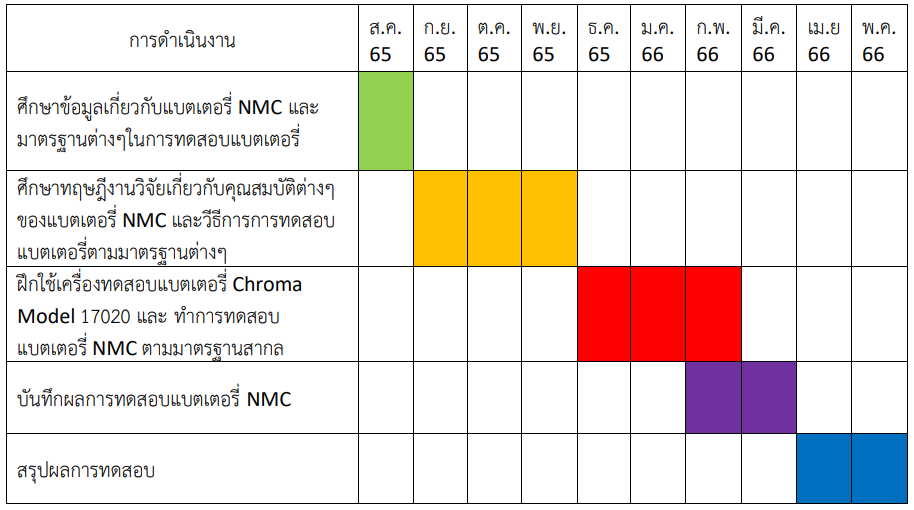
\includegraphics[width=0.8\paperwidth]{Chapters/img/schedule}}
		\centering
		\captionsetup{justification=centering,margin=2cm}
	\end{figure}
\end{center}
%------------------------------------------------------------------------------------------
\section{ประโยชน์ที่คาดว่าจะได้รับ}
\begin{itemize}
  \item ได้รับความรู้และความเข้าใจเกี่ยวกับคุณสมบัติต่างๆของแบตเตอรี่ชนิด NMC
  \item ได้ทักษะการใช้งานเครื่องทดสอบแบตเตอรี่ Chroma Model 17020
  \item ได้ความรู้เกี่ยวกับการทดสอบแบตเตอรี่ตามมาตรฐานที่ได้รับการยอมรับ
  \item ได้นำความข้อมูลจากการทดสอบที่ได้นี้ไปไปประยุกต์ใช้กับยานยนต์ไฟฟ้า
\end{itemize}


